\documentclass[preprint]{sigplanconf}[10pt]

% The following \documentclass options may be useful:
%
% 10pt          To set in 10-point type instead of 9-point.
% 11pt          To set in 11-point type instead of 9-point.
% authoryear    To obtain author/year citation style instead of numeric.

\usepackage{amsmath}
\usepackage{graphicx}
\usepackage{mathpartir} % To use \inferrule
\usepackage{amssymb}    % To use \mathbb

\newtheorem{definition}[section]{Definition}

% Definition of new commands that I use in this text:
\newcommand{\fun}[1]{\mbox{\textbf{#1}}}
\newcommand{\lb}[1]{#1_{\downarrow}}
\newcommand{\ub}[1]{#1_{\uparrow}}
\newcommand{\varset}[1]{\mbox{$\cal{#1}$}}
\newcommand{\code}[1]{\textbf{#1}}

\begin{document}

\conferenceinfo{CGO '13}{February 23 - February 27. Shenzhen, China} 
\copyrightyear{2013}
\copyrightdata{[to be supplied]} 

\titlebanner{Code Generation and Optimization}        % These are ignored unless
\preprintfooter{Dinamica EGO}   % 'preprint' option specified.

\title{An Algorithm to Prune Integer Overflow Tests}
%\subtitle{A case study of the Dinamica EGO toolkit}

\authorinfo{Removed due to blind review}
           {No affiliation given}
           {No e-mail given}

\maketitle

\begin{abstract}
The integer primitive type has upper and lower bounds in many programming
languages, including C, C++ and Java.
This limitation might lead programs that manipulate large integer numbers to
produce unexpected results due to overflows.
There exists a plethora of works that instrument programs to track the occurrence
of these overflows.
In this paper we present an algorithm that relies on static range analysis to
eliminate this instrumentation whenever possible.
We present a novel live range splitting strategy that refine the precision of
our range analysis.
We have used this algorithm to improve the quality of a dynamic instrumentation
library that we have implemented in LLVM.
This framework has been used to detect overflows in hundreds of C/C++ programs.
As a testimony of its effectiveness, our range analysis has been able to speedup
the SPEC CPU 2006 instrumented programs by XX\%.
\end{abstract}

\category{D.3.4}{Processors}{Compilers}

\terms
Languages, Performance

\keywords
Integer arithmetics, Overflow, Compiler, Range analysis

\section{Introduction}
\label{sec:int}

% What are integer overflows.
The most popular programming languages, including C, C++ and Java, limit the
size of primitive numeric types.
For instance, the \texttt{int} type, in Java, ranges from $-2^{31}-1$ to
$2^{31}$.
Consequently, there exist numbers that cannot be represented by these types.
In general, these programming languages resort to a {\em wrapping-arithmetics}
semantics~\cite{TODO} to perform integer operations.
If a number $n$ is too large to fit into a primitive data type $T$, then $n$'s
value wraps around, and $n \mbox{module} T_{max}$ wounds up represented
instead.
There are situations in which this semantics is acceptable~\cite{TODO}.
For instance, programers might rely on this behavior to implement hash functions
and random number generators.
On the other hand, there exist also situations in which this behavior might
lead a program to produce unexpected results.
As an example, in 1996, the Ariane 5 rocket was lost due to an arithmetic
overflow -- a bug that resulted in a loss of more than U\$370 million
dollars~\cite{Dowson97}.
% TODO We need to explain better the wrapping-arithmetics, and we need to cite it
% properly. What could be a good (official) citation?
% And we need to cite

% Why there is still the need to devise efficient methods to eliminate them.
Programming languages such as Ada or Lisp can be customized to throw exceptions
whenever integer overflows are detected.
Furthermore, there exist recent work proposing to instrument binaries derived
from C, C++ and Java programs to detect the occurrence of overflows
dynamically~\cite{Brumley07,Dietz12}.
Thus, if an overflow happens, then the instrumented program can take some
action, such as to log the event, or to terminate the program.
However, this safety comes with a price: arithmetic operations need to be
surveilled, and the runtime checks cost time.
Zhang {\em et al.}~\cite{Zhang09} have proposed to eliminate some of this
overhead via a tainted flow analysis.
We have a similar goal, yet, our approach is substantially different.

% Our contribution: range analysis.
In this paper we discuss a simple and efficient range analysis algorithm that
we have developed to eliminate overflow checks in instrumented programs.
Our algorithm has three core insights.
Firstly, we rely on a three-phases approach to extract information from
comparisons between variables, e.g., $x < y$.
Previous algorithms either deal with these comparisons by resorting to
expensive relational analyses~\cite{Cousot78,Lakhdar11,Mine06}, or only
consider comparisons between variables and
constants~\cite{Mahlke01,Patterson95,Stephenson00}.
Secondly, we rely on strongly connected components to achieve better speed and
precision.
It is well-known that this technique is effective in speeding up static analysis
algorithms~\cite[Sec 6.3]{Nielson99}.
However, given our three-phases approach, we also achieve better precision
by solving strong components in a topological ordering.
Finally, we propose a program representation that allows us to perform a sparse
range analysis while taking benefit from the knowledge that the execution of
an instrumented program is overflow-free.
This extensive live range splitting strategy is only valid if the instrumented
program terminates whenever an integer overflow is detected.
If we cannot rely on this guarantee, then our live range splitting strategy
is more conservative, and produces the program representation that Bodik
{\em et al.}~\cite{Bodik00} have called the Extended Static Single Assignment
form.

% Our experimental results.
We use our range analysis to reduce the runtime overhead imposed by a dynamic
instrumentation library.
This instrumentation framework, also a contribution of this paper, has been
implemented in the LLVM compiler~\cite{Lattner04}.
We have used it to log overflows in a vast number of programs, and in this
paper we focus on SPEC CPU 2006.
Our implementation has been able to reproduce the results recently obtained by XX
{\em et al.}~\cite{TODO}.
Our range analysis algorithm has been able to remove XX\% of the overflow
checks created by the dynamic instrumentation framework.
All our experiments use an interprocedural version of range analysis.
We inline small functions to make our implementation more context sensitive.
Our experiments show that the speed and memory consumption of our range analysis
grows linearly with the program size.
By comparing the ranges that we determine statically with the results found by
a profiler, we see that more than 50\% of the bounds that we found are within a
factor of 50\% of the values that variables actually assume.

\subsection{The Danger that Integer Overflows Represent}
\label{sub:danger}

% A brief overview about integer overflows.
In addition to being a source of several bugs that are hard to identify, integer 
overflows can represent a serious security risk.
As pointed by Dietz {\em et al.}~\cite{Dietz12}, integer overflows are the
sources of vulnerabilities in widely used software, such as OpenSSH and
Firefox.
These vulnerabilities could give an adversary the opportunity to execute
arbitrary code in the compromised application. 
We will demonstrate this with an example.
The $n$-bits two's complement arithmetics wraps around at multiples of
$2^n$.
As an example the representation of $16 \times 16$ in 8-bits two's complement
is $0$, because $0 \equiv (16\times16) \mod 2^8$.
Programmers can use this well-defined behavior in benign ways.
For instance, the wrapping arithmetics provides a cheap $\mod 2^n$ operator,
which is used in the implementation of hash-functions or random number
generators.

\begin{figure}[t!]
\begin{center}
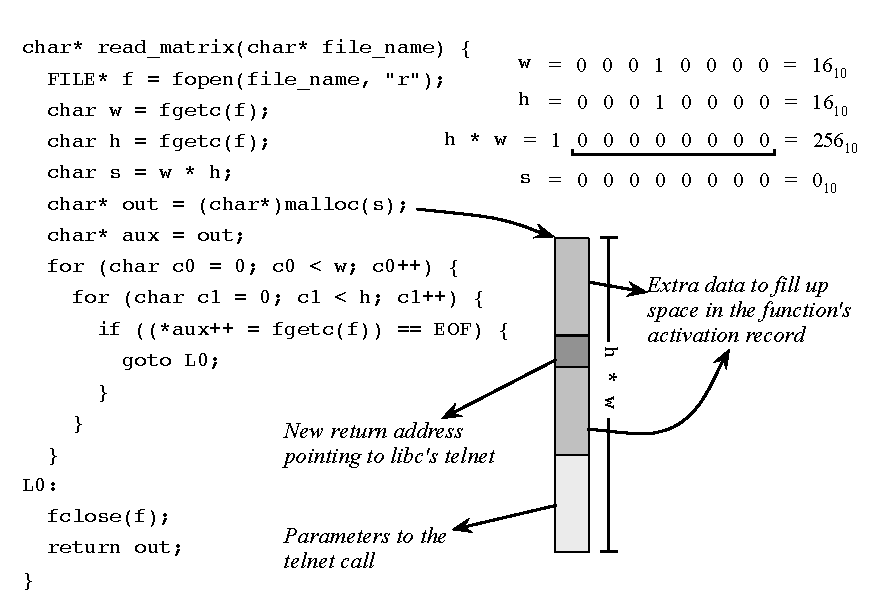
\includegraphics[width=\columnwidth]{images/ex_buffer_overflow}
\end{center}
\caption{\label{fig:ex_buffer_overflow}
An example of an exploitable integer overflow vulnerability.}
\end{figure}

% An example of vulnerability.
Figure~\ref{fig:ex_buffer_overflow} illustrates an example of integer
overflow vulnerability.
This vulnerability allows an adversary to perform a buffer overrun attack
on a program that is apparently guarded against this type of exploit.
For simplicity, we will use the C datatype \texttt{char}, which represents
8-bit long numbers.
Examples of actual vulnerabilities, with larger primitive types, are given
by Brumley {\em et al.}~\cite{Brumley07}, Dietz {\em et al.}~\cite{Dietz12}, and
Zhang {\em et al.}~\cite{Zhang09}.
The function \texttt{read\_matrix} reads a matrix of bytes from a file.
This matrix is stored as a linear sequence of bytes in a vector \texttt{out}.
The first and second bytes in the file, e.g., \texttt{w} and \texttt{h},
determine the number of rows and columns in the matrix.
If the \texttt{char} datatype could represent arbitrarily long numbers, than this
function would be safe against buffer overruns, because it would only write data
on allocated memory.
However, if, for instance, we have that \texttt{w}$= 16$ and \texttt{h}$= 16$,
then \texttt{s}$= 0$, as pointed before.
In this case, a buffer of length zero would be allocated, and all the data
stored in the file would overwrite memory in the stack of activation records.
By carefully crafting an input file, and adversary can, in this way, overwrite
the return address of \texttt{read\_matrix}, diverting program's execution to
one of \texttt{libc}'s function, such as \texttt{telnet}, for instance.

\section{Range Analysis}
\label{sec:range}

\subsection{The Interval Lattice}
\label{sub:lattice}

% Define the lattice, the constraints and the valuation I.
Following Gawlitza {\em et al.}'s notation~\cite{Gawlitza09}, we shall be
performing arithmetic operations over the complete lattice
$\cal{Z} = \mathbb{Z} \cup \{-\infty, +\infty\}$, where the ordering is
naturally given by $-\infty < \ldots < -2 < -1 < 0 < 1 < 2 < \ldots +\infty$.
For any $x > -\infty$ we define:

\begin{tabular}{lcl}
$x + \infty = \infty, x \neq -\infty$ & \mbox{\hspace{0.1cm}} & $x - \infty = - \infty, x \neq +\infty$ \\
$x \times \infty = \infty$ if $x > 0$ & & $x \times \infty = -\infty$ if $x < 0$ \\
$0 \times \infty = 0$ & & $(-\infty) \times \infty = \ $ not defined $$ \\
\end{tabular}

From the lattice $\varset{Z}$ we define the product lattice
$\varset{Z}^2$, which is defined as follows:
%
\begin{equation*}
\varset{Z}^2 = \{ \emptyset \} \cup \{[z_1, z_2] | \ z_1,z_2 \in \varset{Z},
\ z_1 \leq z_2, \  -\infty < z_2 \}
\end{equation*}
%
This interval lattice is partially ordered by the subset relation, which we
denote by ``$\sqsubseteq$".
Range intersection, ``$\sqcap$", is defined by:
\[
[a_1, a_2] \sqcap [b_1, b_2] =
\begin{cases}
[\mbox{max}(a_1, b_1), \mbox{min}(a_2, b_2)], \ \mbox{if} \ a_1 \leq b_1 \leq a_2  \\ \mbox{or} \ b_1 \leq a_1 \leq b_2 \\
[a_1, a_2] \sqcap [b_1, b_2] = \emptyset, \ \mbox{otherwise}
\end{cases}
\]
And range union, ``$\sqcup$", is given by:
\[
[a_1, a_2] \sqcup [b_1, b_2] = [\mbox{min}(a_1, b_1), \mbox{max}(a_2, b_2)]
\]

Given an interval $\iota = [l, u]$, we let $\lb{\iota} = l$, and
$\ub{\iota} = u$.
We let \varset{V} be a set of constraint variables, and
$I: \varset{V} \mapsto \varset{Z}^2$ a
mapping from these variables to intervals in $\varset{Z}^2$.
Our objective is to solve a constraint system $C$, formed by constraints such
as those seen in Figure~\ref{fig:eval_function}(left).
We let the $\phi$-functions be as defined by Cytron
{\em et al.}~\cite{Cytron91}: they join different variable names into a single
definition.
Figure~\ref{fig:eval_function}(right) defines a valuation function $e$ on the
interval domain.
Armed with these concepts, we define the range analysis problem as follows:

\begin{definition}
\label{def:rcp}
\textsc{Range Analysis Problem} \\
\textbf{Input:} a set $C$ of constraints ranging over a set \varset{V} of
variables. \\
\textbf{Output:} a mapping I such that, for any variable
$V \in \varset{V}$, e(V) = I[V].
\end{definition}

\begin{figure}[t!]
\begin{center}
\begin{small}
\begin{eqnarray*}
\begin{array}{r@{\hspace{.5cm}}c}
Y = [l, u]
&
e(Y) = [l, u]
\\
\\
Y = \phi (X_1, X_2)
&
\inferrule{I[X_1]=[l_1, u_1] \\ I[X_2]=[l_2, u_2]}
{e(Y) = [l_1, u_1] \sqcup [l_2, u_2]}
\\
\\
Y = X_1 + X_2
&
\inferrule{I[X_1]=[l_1, u_1] \\ I[X_2]=[l_2, u_2]}
{e(Y) = [l_1 + l_2, u_1 + u_2]}
\\
\\
Y = X_1 \times X_2
&
\inferrule{L = \{l_1l_2, l_1u_2, u_1l_2, u_1u_2\} \\ I[X_1]=[l_1, u_1] \\ I[X_2]=[l_2, u_2]}
{e(Y) = [\mbox{min}(L), \mbox{max}(L)]}
\\
\\
Y = aX + b
&
\inferrule{I[X]=[l, u] \\ k_l = al + b \\ k_u = au + b}
{e(Y) = [\mbox{min}(k_l, k_u), \mbox{max}(k_l, k_u)]}
\\
\\
Y = X \sqcap [l', u']
&
\inferrule{I[X]=[l, u]}
{e(Y) \leftarrow [l, u] \sqcap [l', u']}
\end{array}
\end{eqnarray*}
\caption{\label{fig:eval_function}
A suite of constraints that produce an instance of the range analysis problem.}
\end{small}
\end{center}
\end{figure}

We will use the program in Figure~\ref{fig:ex1}(a) to illustrate our range
analysis.
Figure~\ref{fig:ex1}(b) shows the same program in e-SSA form~\cite{Bodik00},
and Figure~\ref{fig:ex1}(c) outlines the constraints that we extract from this
program.
There is a clear correspondence between instructions and constraints.
Our analysis is sparse~\cite{Choi91}; thus, we associate one, and only one,
constraint with each integer variable defined in the program.
A possible solution to the range analysis problem, as obtained via the
techniques that we will introduce in Section~\ref{sub:algo}, is given in
Figure~\ref{fig:ex_eSSA_cgo}(d).

\begin{figure}[t!]
\begin{center}
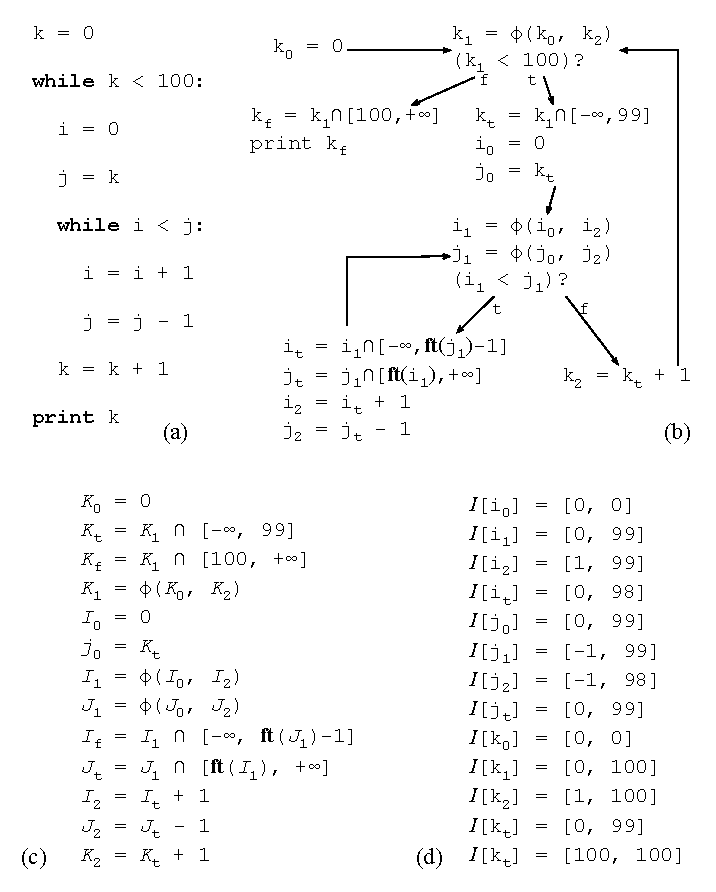
\includegraphics[width=\columnwidth]{images/ex_eSSA_cgo}
\end{center}
\caption{\label{fig:ex_eSSA_cgo}
(a) Example program.
(b) Control Flow Graph in SSA form.
(c) Constraints that we extract from the program.
(d) Possible solution to the range analysis problem.}
\end{figure}

\subsection{Range Propagation}
\label{sub:prop}

% The macro algorithm
The range analysis algorithm that we propose in this paper works in a number
of steps.
Firstly, we convert the program to an intermediate representation that gives
us subsidies to perform a sparse analysis.
We have tested our algorithm with two different representations, as we discuss
in Section~\ref{sub:splitting}.
Secondly, we extract constraints from the program representation.
Thirdly, we build a constraint graph, following the strategy pointed by
Su and Wagner~\cite{Su05}.
However, contrary to them, in a next phase we find the strongly connected
components in this graph, collapse them into super-nodes, and sort the
resulting digraph topologically.
Finally, for each strong component, we apply a three-phases approach to determine
the ranges of the variables.

\noindent
\textbf{Building the Constraint Graph. }
Given a set $\varset{C}$ of constraints, which define and/or use constraint
variables from a set $\varset{V}$, we build a constraint graph
$G = (\varset{C} \cup \varset{V}, E)$.
We call the vertices in \varset{C} the {\em constraint nodes}, and we call the
nodes in \varset{V} the {\em variable nodes}.
If variable $V \in \varset{V}$ is used in constraint $C \in \varset{C}$, then
we create an edge from $V$ to $C$.
If constraint $C \in \varset{C}$ defines variable $\varset{V} \in V$, then we
create an edge from $C$ to $V$.
Figure~\ref{fig:ex_graph} shows the constraint graph that we build for the
program in Figure~\ref{fig:ex_eSSA_cgo}(b).
If $V$ is used by $C$ as the input of a future, then the edge from
$V$ to $C$ represents what Ferrante {\em et al.} call a {\em control
dependence}~\cite[p.323]{Ferrante87}.
We use dashed lines to represent these edges.
All the other edges denote {\em data dependences}~\cite[p.322]{Ferrante87}.
As we will show later, control dependence edges increase the precision of our
algorithm to solve future bounds.

\begin{figure}[t!]
\begin{center}
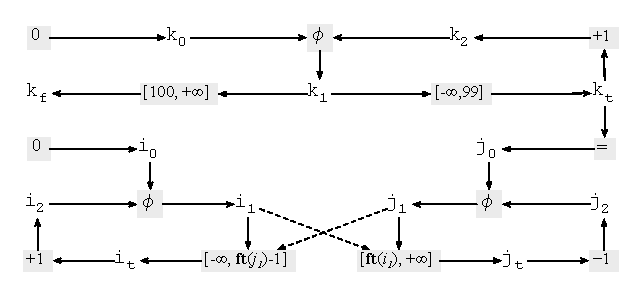
\includegraphics[width=\columnwidth]{images/ex_graph}
\end{center}
\caption{\label{fig:ex_graph}
The constraint graph that we build to the program in
Figure~\ref{fig:ex_eSSA_cgo}(b).}
\end{figure}

\noindent
\textbf{Propagating Ranges in Topological Order. }
After building the constraint graph, we find its strongly connected components.
We collapse these components in super nodes, and then proceed to propagate
ranges along the resulting digraph.
This approach is essential for scalability, because all the complexity of our
algorithm lies in the resolution of strong components.
Our tests show that the vast majority of the strongly connected components are
singletons.
For instance, 99.11\% of the SCCs in SPEC CPU 2006 gcc (\texttt{403.gcc}) have
only one node.
Moreover, the composite components usually contain a small number of nodes.
As an example, the largest component in \texttt{403.gcc}, has 2,131 nodes,
even though gcc's constraint graph has over one million nodes.
This large SCC exists due to a long chain of mutually recursive function calls.

\subsection{A Three-Phases Approach to Solve Strong Components}
\label{sub:micro}

We determine the ranges for each strongly connected component in a three phases
approach.
For each SCC, first we determine the growth pattern of each variable via a
widening phase.
In the second step, once we know in which directions the values stored in each
variable might grow, we replace futures by actual bounds.
Finally, we have a narrowing phase that uses conditional tests to improve the
precision of our results.

\noindent
\textbf{Widening: } we start solving constraints by determining how each program
variable might grow.
For instance, if a variable is only updated by sums with positive numbers, then
we say that it only grows up.
If, instead, a variable is only updated by sums with negative numbers, then it
grows down.
Some variables can also grow in both directions.
We discover these growth patterns by abstractly interpreting the constraints that
constitute the strongly connected component.
We ensure termination via a widening operator.
Our implementation uses {\em jump-set widening}, which is typically used in
range analysis~\cite[p.228]{Nielson99}.
This operator is a generalization of Cousot and Cousot's original widening
operator~\cite{Cousot77}, which we describe below:
%
\begin{equation*}
I[Y] =
\begin{cases}
\mbox{if} \ I[Y] = [\bot, \bot] \ \mbox{then} \ e(Y) \\
\mbox{elif} \ \lb{e(Y)} < \lb{I[Y]}  \ \mbox{and} \ \ub{e(Y)} > \ub{I[Y]} \ \mbox{then} \ [-\infty, \infty] \\
\mbox{elif} \ \lb{e(Y)} < \lb{I[Y]} \ \mbox{then} \ [-\infty, \ub{I[Y]}] \\
\mbox{elif} \ \ub{e(Y)} > \ub{I[Y]} \ \mbox{then} \ [\lb{I[Y]}, \infty]
\end{cases}
\end{equation*}
%
We let $\lb{[l, u]} = l$ and $\ub{[l, u]} = u$.
The map $I$ and the abstract evaluation function $e$ are determined as in
Figure~\ref{fig:eval_function}.
We have a different implementation of $e$ for each operation that the
target programming language provides.
Our current LLVM implementation has 18 different instances of $e$, including
signed and unsigned addition, subtraction, multiplication and division, plus
truncation, the bitwise integer operators and $\phi$-functions.

If we use the widening operator above, then the abstract state of any constraint
variable can only change three times, e.g., $[\bot, \bot] \rightarrow [c_1, c_2]
\rightarrow [c_1, \infty] \rightarrow [-\infty, \infty]$, or
$[\bot, \bot] \rightarrow [c_1, c_2] \rightarrow [-\infty, c_2]
\rightarrow [-\infty, \infty]$.
Therefore, we can determine the growth behavior of each constraint variable in
a strong component in linear time on the number of constraints in that
component.
Figure~\ref{fig:ex_partition_grow_crop}(b) shows the abstract state of the
variables in the largest SCC of the graph in Figure~\ref{fig:ex_graph}.
As we see in the figure, this step of our algorithm has been able to determine
that variables \texttt{i}$_1$, \texttt{i}$_2$ and \texttt{i}$_t$ can only
increase, and that variables \texttt{j}$_1$, \texttt{j}$_2$ and \texttt{j}$_t$
can only decrease.

\begin{figure}[t!]
\begin{center}
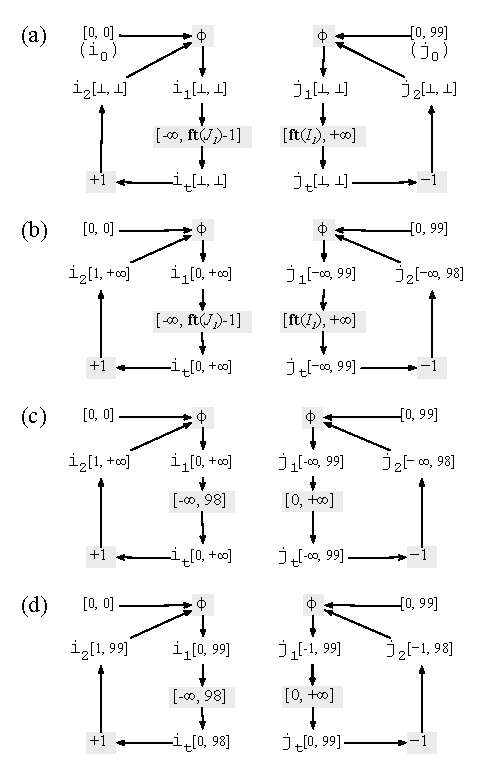
\includegraphics[width=0.9\columnwidth]{images/ex_partition_grow_crop}
\end{center}
\caption{\label{fig:ex_partition_grow_crop}
Four snapshots of the last SCC of Figure~\ref{fig:ex_graph}.
(a) After removing control dependence edges.
(b) After running the growth analysis.
(c) After fixing the intersections bound to futures.
(d) After running the narrowing analysis.}
\end{figure}

\noindent
\textbf{Future resolution: }
The next phase of the algorithm to determine intervals inside a strong
component consists in replacing futures by actual bounds, a task that we
accomplish by using the rules below:
%
\begin{eqnarray*}
\begin{array}{c}
\inferrule{Y = X \sqcap [l, \fun{ft}(V) + c] \\ \ub{I[V]} = u}
{Y = X \sqcap [l, u + c]} \mbox{\hspace{0.3cm}} u, c \in \mathbb{Z} \cup \{-\infty, \infty\}
\\
\\
\inferrule{Y = X \sqcap [\fun{ft}(V) + c, u] \\ \lb{I[V]} = l}
{Y = X \sqcap [l + c, u]} \mbox{\hspace{0.3cm}} l, c \in \mathbb{Z} \cup \{-\infty, \infty\}
\end{array}
\end{eqnarray*}
%
In order to correctly replace a future $\fun{ft}(V)$ that limits a constraint
variable $V'$, we need to have already applied the growth analysis onto $V$.
Had we considered only data dependence edges, then it would be possible
that $V'$ be analyzed before $V$.
However, because of control dependence edges, this case cannot happen.
The control dependence edges ensure that any topological ordering of the
constraint graph either places $V$ before $V'$, or places these nodes
in the same strongly connected component.
For instance, in Figure~\ref{fig:ex_graph}, variables $j_1$ and $i_t$ are in
the same SCC only because of the control dependence edges.
Figure~\ref{fig:ex_partition_grow_crop}(c) shows the result of resolving
futures in our running example.
The information that we acquire from the growth analysis is essential in this
phase.
For instance, the growth analysis has found out that the value stored in variable
\texttt{i}$_i$ can only increase.
Given that this variable is assigned the initial value zero, we can replace
$\fun{ft}(I_1)$ with this value.

\noindent
\textbf{Narrowing: } the last step that we apply on the strongly connected
component is the narrowing phase.
In this step we use values extracted from conditional tests to restrict the
bounds of the constraint variables.
We use the narrowing operator firstly proposed by Cousot and
Cousot~\cite{Cousot77}, which we show below:
%
\begin{equation*}
I[Y] =
\begin{cases}
\mbox{if} \ \lb{I[Y]} = -\infty  \ \mbox{and} \ \lb{e(Y)} > -\infty \ \mbox{then} \ [\lb{e(Y)}, \ub{I[Y]}] \\
\mbox{elif} \ \ub{I[Y]} = \infty \ \mbox{and} \ \ub{e(Y)} < \infty \ \mbox{then}
\ [\lb{I[Y]}, \ub{e(Y)}] \\
\mbox{elif} \ \lb{I[Y]} > \lb{e(Y)} \ \mbox{then} \ [\lb{e(Y)}, \ub{I[Y]}] \\
\mbox{elif} \ \ub{I[Y]} < \ub{e(Y)} \ \mbox{then} \ [\lb{I[Y]}, \ub{e(Y)}]
\end{cases}
\end{equation*}
%
Figure~\ref{fig:ex_partition_grow_crop}(d) show the result of our narrowing
operator in our running example.
Ranges initially improve due to the two conditional tests in the program.
Firstly, we have that $I[I_t] = I[I_1] \sqcap [-\infty, 98]$, which gives us
that $I[I_t] = [0, 98]$.
We also have that $I[J_t] = I[J_1] \sqcap [0, \infty]$, giving
$I[J_t] = [0, 99]$.
From these new intervals, we can narrow the ranges bound to the other constraint
variables.

The combination of widening, futures and narrowing, plus use of strong components
gives us, in this example, a very precise solution.
We emphasize that finding this tight solution was only possible because of
the topological ordering of the constraint graph in Figure~\ref{fig:ex_graph}.
Upon meeting the constraint graph's last SCC, shown in
Figure~\ref{fig:ex_partition_grow_crop}, we had already determined that the
interval $[0, 0]$ is bound to $i_0$ and that the interval $[0, 99]$ is bound to
$j_0$, as we show in Figure~\ref{fig:ex_partition_grow_crop}(a).
Had we applied the widening operator onto the whole graph, then we would
have found out that variable $j_1$ is bound to $[-\infty, +\infty]$.
This imprecision happens because, on one hand $j_1$'s interval is influenced
by $k_t$'s, which is upper bounded by $+\infty$.
On the other hand $j_1$ is part of a decreasing cycle of dependences formed by
variables $j_t$ and $j_2$ in addition to itself.
Therefore, if we had applied the widening phase over the entire program followed
by a global narrowing phase, then we would not be able to recover some of
widening's precision loss.
However, because in this example we only analyze $j$'s SCC after we have
analyzed $k$'s, $k$ only contribute the constant range $[0, 99]$ to $j_0$.


\subsection{Live Range Splitting Strategies}
\label{sub:splitting}

A dense dataflow analysis associates information, i.e., a point in a lattice,
with each pair formed by a variable plus a program point.
If this information is invariant along every program point where the variable
is alive, then we can associate the information with the variable itself.
In this case, we say that the dataflow analysis is {\em sparse}~\cite{Choi91}.
A dense dataflow analysis can be transformed into a sparse one via a suitable
intermediate representation.
A compiler builds this intermediate representation by splitting the live ranges
of variables at the program points where the information associated with these
variables might change.
To split the live range of a variable $v$, at a program point $p$, we insert
a copy $v' = v$ at $p$, and rename every use of $v$ that is dominated by $p$.
In this paper we have experimented with two different live range splitting
alternatives.

The first strategy is the {\em Extended Static Single Assignment} (e-SSA) form,
proposed by Bodik {\em et al.}~\cite{Bodik00}.
We build the e-SSA representation by splitting live ranges at definition sites
-- hence it subsumes the SSA form -- and at conditional tests.
The program in Figure~\ref{fig:ex_eSSA_cgo}(b) is in e-SSA form.
Let $(v < c)?$ be a conditional test, and let $l_t$ and $l_f$ be labels in
the program, such that $l_t$ is the target of the test if the condition is true,
and $l_f$ is the target when the condition is false.
We split the live range of $v$ at any of these points if at least one of two
conditions is true:
(i) $l_f$ or $l_t$ dominate any use of $v$;
(ii) there exist a use of $v$ at the dominance frontier of $l_f$ or $l_t$.
For the notions of dominance and dominance-frontier, see Aho
{\em et al.}~\cite[p.656]{Aho06}.
To split the live range of $v$ at $l_f$ we insert at this
program point a copy $v_f = v \sqcap [c, +\infty]$, where $v_f$ is a fresh name.
We then rename every use of $v$ that is dominated by $l_f$ to $v_f$.
Dually, if we must split at $l_t$, then we create at this point a copy
$v_t = v \sqcap [-\infty, c-1]$, and rename variables accordingly.
If the conditional uses two variables, e.g., $(v_1 < v_2)?$, then we create
intersections bound to {\em futures}.
We insert, at $l_f$, $v_{1f} = v_1 \sqcap [\fun{ft}(v_2), +\infty]$,
and $v_{2f} = v_2 \sqcap [-\infty, \fun{ft}(v_1)]$.
Similarly, at $l_t$ we insert
$v_{1v} = v_1 \sqcap [-\infty, \fun{ft}(v_2) - 1]$
and $v_{2f} = v_2 \sqcap [\fun{ft}(v_1) + 1, +\infty]$.
Notice that a variable $v$ can never be associated with a future bound to
itself, e.g., $\fun{ft}(v)$.
This invariant holds because whenever the e-SSA conversion associates a variable
$u$ with $\fun{ft}(v)$, then $u$ is a fresh name created to split the live range
of $v$, given that $v$ was used in a conditional.

The second intermediate representation consists in splitting live ranges at
(i) definition sites -- it subsumes SSA, (ii) at conditional tests -- it
subsumes e-SSA, and at some use sites.
This representation, which we henceforth call u-SSA, is only valid if we
assume that integer overflows cannot happen.
We can provide this guarantee by using our dynamic instrumentation to terminate
a program in face of an overflow.
The rationale behind u-SSA is as follows: we know that past an instruction such
as $v = u + c, c \in \mathbb{Z}$ at a program point $p$, variable $u$ must be
less than $\mathit{MaxInt} - c$.
If that were not the case, then an overflow would have happened and the
program would have terminated.
Therefore, we split the live range of $u$ past its use point $p$, producing the
sequence $v = u + c; u' = u$, and renaming every use of $u$ that is dominated
by $p$ to $u'$.
We then associate $u$ with the constraint $I[U'] \sqsubseteq I[U] \sqcap [-\infty, \mathit{MaxInt} - c]$.

\begin{figure}[t!]
\begin{center}
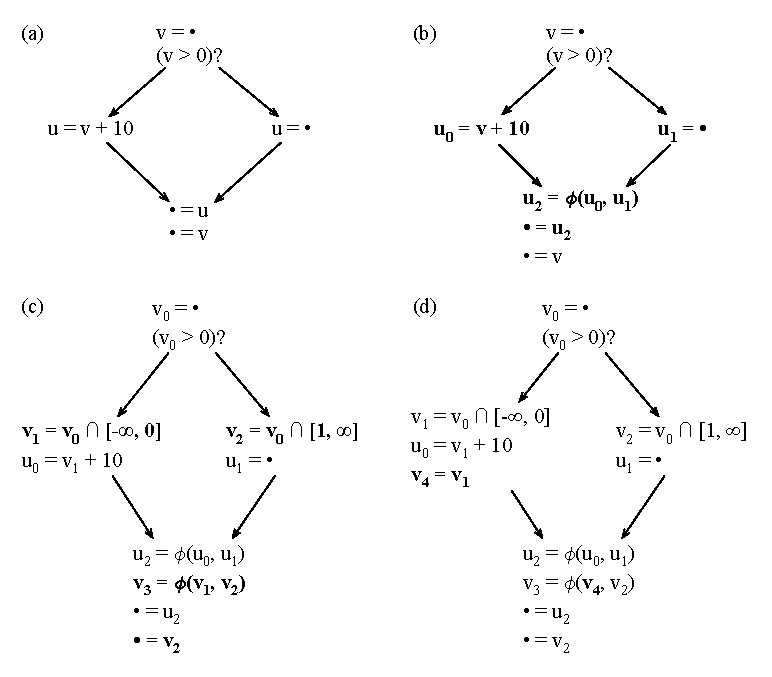
\includegraphics[width=\columnwidth]{images/ex_ir}
\end{center}
\caption{\label{fig:ex_ir}
(a) Example program.
(b) SSA form~\cite{Cytron91}.
(c) e-SSA form~\cite{Bodik00}.
(d) u-SSA form.}
\end{figure}

Figure~\ref{fig:ex_ir} compares the u-SSA form with the SSA and e-SSA
intermediate program representations.
We use the notation $v = \bullet$ to denote a definition of variable $v$, and
$\bullet = v$ to denote a use of that variable.
Figure~\ref{fig:ex_ir}(b) shows the example program converted to the SSA format.
The different definitions of variable $u$ have been renamed, and a
$\phi$-function re-combines these definitions into a single name.
The SSA form sparsifies a dataflow analysis that only extracts information from
the definition sites of variables, such as constant propagation.
Figure~\ref{fig:ex_ir}(c) shows the same program in e-SSA form.
This time we have renamed variable $v$ right after the conditional test where
this variable is used.
The e-SSA form serves dataflow analyses that acquire information from definition
sites and conditional tests.
Examples of these analyses include array bounds checking
elimination~\cite{Bodik00} and traditional implementations of range
analyses~\cite{Gough94,Patterson95}.
Finally, Figure~\ref{fig:ex_ir}(d) shows our example in u-SSA form.
The live range of variable $v_1$ has been divided right after its use.
This representation is useful to analyses that learn information from the way
that variables are used, and propagate this information forwardly.

\section{The Dynamic Instrumentation Library}
\label{sec:dyn}

%What is our instrumentation library
We have implemented our instrumentation library as a LLVM transformation pass.
This means our library works on the LLVM IR\footnote{LLVM Intermediate Representation, available at \url{http://llvm.org/docs/LangRef.html}}
instead of working directly on the original source code. 
This fact brings the advantage of allowing us to rely on
other analysis, such as the range analysis, to check if it is safe to state that
the possible values of an instruction will always be within the range of
the declared type of the instruction. 
If we can state this, it means that it is impossible for an overflow to 
occur in the analyzed instruction, because the range analysis is a conservative analysis; 
in this case, we don't need to insert dynamic checks, and the instrumented program
will be smaller and run faster than it would run without this prunning.
%How our instrumentation works
Our instrumentation works by identifying the instructions that may 
lead to an overflow, and inserting assertions after that instructions. 
The LLVM IR has five instructions that may lead to an overflow: 
ADD, SUB, MUL, SHL, and TRUNC.

%ADD instrumentation
The ADD instruction performs the sum of two operands $op_1$ and $op_2$ and
stores the result in a variable $x$.
The semantics of an ADD instruction is $x = op_1 + op_2$. 
The goal of the instrumentation of the instruction $x$ is to ensure that after the
execution of the ADD instruction, $x$ stores the correct result of the sum,
without any data loss.
For this, we insert different checks for signed and unsigned instructions.
If we are dealing with an unsigned ADD instruction $x$, we insert the following check:
\code{if $x < op_1$ or $x < op_2$ then} handle overflow \code{else} continue to 
$x$'s next instruction. If, instead, we are instrumenting a signed instruction $x$, 
we will have the following assertion:
\code{if ($op_1 > 0$ and $op_2 > 0$ and $x < 0$) or ($op_1 < 0$ and $op_2 < 0$ and $x > 0$) then} 
handle overflow \code{else} continue to $x$'s next instruction.

%SUB instrumentation
The SUB instruction performs the subtraction of two operands $op_1$ and $op_2$ and
stores the result in a variable $x$.
The semantics of an SUB instruction is $x = op_1 - op_2$. 
Note that the SUB semantics is close to the ADD semantics. For this reason, the
instrumentation of the SUB instructions looks like the ADD instrumentation.
In this case, we insert different checks for signed and unsigned instructions, too.
If we are dealing with an unsigned SUB instruction $x$, we insert the following check:
\code{if $op_1 < op_2$ then} handle overflow \code{else} continue to 
$x$'s next instruction. Note that the assertion makes a single comparison. This is sound
because if $op_2$ is greater than $op_1$, the result would be negative. However, unsigned
integers can't represent negative numbers. In this case, we have a overflow.
The instrumentation of a signed SUB instruction $x$ will have the following assertion:
\code{if ($op_1 < 0$ and $op_2 > 0$ and $x > 0$) or ($op_1 > 0$ and $op_2 < 0$ and $x < 0$) then} 
handle overflow \code{else} continue to $x$'s next instruction.

%MUL instrumentation
The MUL instruction performs the multiplication of two operands $op_1$ and $op_2$ and
stores the result in a variable $x$.
The semantics of an SUB instruction is $x = op_1 \times{} op_2$. 
The dynamic check of the MUL instruction is the same for signed or unsigned
instructions, because it relies on DIV, the inverse operation. 
To verify if the overflow has occurred, we divide $x$ by $op_1$. If the result
is different of $op_2$, then we have an overflow to handle. 
In this case, we will have the following assertion: 
\code{if $op_1 \neq{} 0$ and $(x \div{} op_1) \neq{} op_2$ then} 
handle overflow \code{else} continue to $x$'s next instruction.
Note that if $op_1 = 0$, the result of the multiplication will never overflow,
because the result of the MUL will be $0$, too. In this case, if $op_1 \eq{} 0$,
we don't perform the DIV, to prevent a division by zero exception.
This technique of using the inverse operation to check for overflows doesn't work
for ADD and SUB instructions because the $n$-bits two's complement wrapping-arithmetics 
would give us false negatives in the assertions.

%SHL instrumentation
The SHL instruction performs the shift left operation. It receives a value $op_1$
and the number of bits $n$ the SHL will shift $op_1$ by; the operation's result
is stored in a variable $x$.
The semantics os a SHL instruction is $x = op_1 \times{} 2^n$. 
The SHL instructions result in overflows when the $op_1$ is positive and 
$x$ is negative or when $op_1$ is negative and $n \neq{} 0$, because 
the SHL in negative numbers would produce undefined results that are
as harmful as integer overflows. This assertion has the same semantics for
signed and unsigned instructions.
In this case, we will have the following check: 
\code{if ($op_1 > 0$ and $x < op_1$) or ($op_1 < 0$ and $n \neq{} 0$) then} 
handle overflow \code{else} continue to $x$'s next instruction.

%TRUNC instrumentation
The TRUNC instruction performs the truncation of the operand $op_1$
to a number $n$ of bits and stores the result in a variable $x$.
The semantics of a TRUNC instruction is $x = n$LessSignificantBits$(op_1)$.
The dynamic checking of a TRUNC instruction is done by expanding $x$ to
the datatype of $op_1$ and comparing the expanded $x$ with $op_1$. If they 
don't have the same value, some data has been lost by the TRUNC instruction.
In this case, we have the following check:
\code{if $cast(x, getDataType(op_1)) \neq{} op_1$ then} 
handle overflow \code{else} continue to $x$'s next instruction.
Note that the instrumentation of the TRUNC instructions is a very fragile point, 
because it would catch any truncation with loss of precision, even if it is a
benign one.
To avoid trouble and make it easier to our users, the instrumentation library 
can receive an argument to let the user decide whether to insert or not
instrumentation in the TRUNC instructions.

%Overview about the instrumentation technique
Our instrumentation library works by adding new instructions to
the target programs. The instrumentation of all the instructions works
in the same way: first, the pass inserts instructions to gather the
information needed to do the assertion.
Then, the pass inserts compare instructions to generate a boolean value
that indicates if there is an overflow or not. 
After this, the pass inserts a conditional branch: 
the false clause of the branch, where the control goes when there is no 
overflow and the program, leads to the first instruction after the instruction
which has received the instrumentation.
the true clause of the branch leads to a block where we do the
overflow handling. 

%What we can do in the overflow handling
Our library has three options to handle the overflows. 
First option: Do nothing and ignore the overflows. This option
was used to do our experiments and verify the slowdown produced 
by the new instructions.
Second option: Give a message in stderr whenever an overflow occurs.
This is the standard option. The instrumented program remains with 
the same behavior, but whenever an overflow occurs, the program
prints \texttt{Overflow occurred in FileName.cpp, line X.} in the
standard error stream.
Third option: Abort the execution when an overflow occurs.
This is the more aggressive option. With this option enabled,
whenever an overflow occurs, the program is terminated, not allowing
the execution of the program with undefined behavior due to 
integer overflows.

\section{Experimental Results}
\label{sec:exp}

We have implemented our range analysis algorithm in LLVM 3.0, and have run
experiments on a Intel quad core CPU with a 2.40GHz clock, and 3.6GB of RAM.
Each core has a 4,096KB L1 cache.
We use Linux Ubuntu 10.04.4.
Our implementation of range analysis has 3,958 lines of
commented C++ code, our e/u-SSA conversion module has 672 lines, and our
instrumentation pass has 762 lines.
We have analyzed 428 C programs that constitute the LLVM test suite plus the
integer benchmarks in SPEC CPU 2006.
Together, these programs contain 4.76 million assembly instructions.
This section has two main goals.
First, we want to show that our range analysis is fast and precise.
Second, we want to demonstrate the effectiveness of our framework to detect
integer overflows.

\noindent
\textbf{Time and Memory Complexity.}
Figure~\ref{fig:TimeCorr} provides a visual comparison between the time to
run our range analysis and the size of the input programs.
We show data for the 100 largest benchmarks in our test suite, in number
of variable nodes in the constraint graph.
We perform function inlining before running our analysis.
Each point in the X line corresponds to a benchmark.
We analyze the smallest benchmark in this set, \texttt{Prolangs-C/deriv2}, which
has 1,131 variable nodes in the constraint graph, in 20ms.
We take 15.91 sec to analyze our largest benchmark, \texttt{403.gcc}, which,
after function inlining, has 1,266,273 assembly instructions, and a
constraint graph with 679,652 variable nodes.
For this data set, the coefficient of determination $(R^2)$ is 0.967, which
provides very strong evidence about the linear asymptotic complexity of our
implementation.

\begin{figure}[t!]
\begin{center}
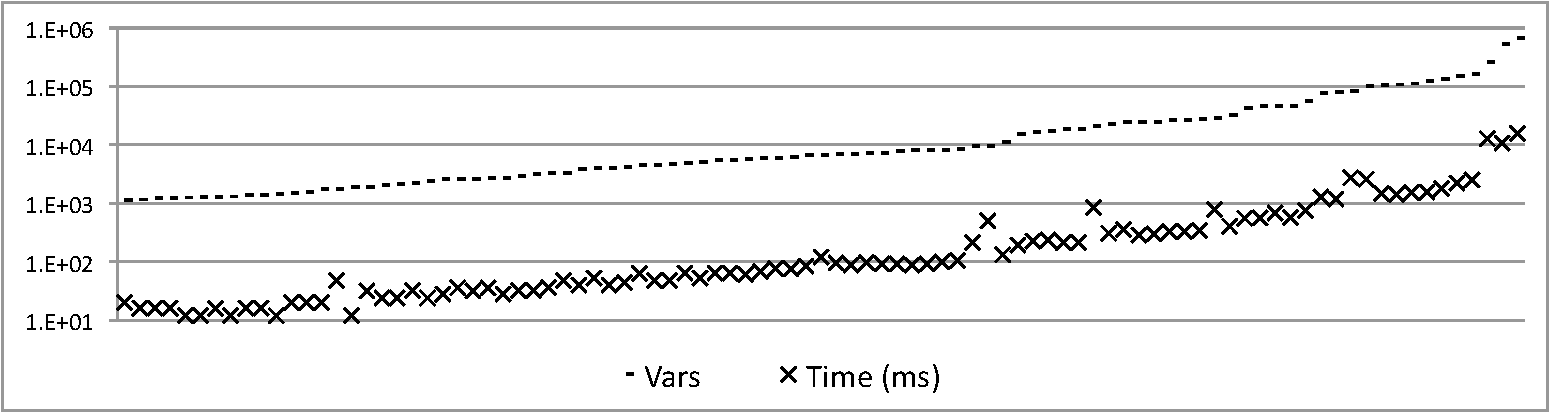
\includegraphics[width=\columnwidth]{images/TimeCorr}
\end{center}
\caption{\label{fig:TimeCorr}
Correlation between program size (number of var nodes in constraint
graphs after inlining) and analysis runtime (ms).
Coefficient of determination = 0.967.
}
\end{figure}

The experiments also reveal that the memory consumption of our implementation
is linear with the program size.
Figure~\ref{fig:MemCorr} plots these two quantities together.
The linear correlation, in this case, is even stronger than that found in
Figure~\ref{fig:TimeCorr}, which compares runtime and program size: the
coefficient of determination is 0.9947.
The figure only shows our 100 largest benchmarks.
Again, SPEC \texttt{403.gcc} is the heaviest benchmark, requiring
265,588KB to run.
Memory includes stack, heap and the executable program code.

\begin{figure}[t!]
\begin{center}
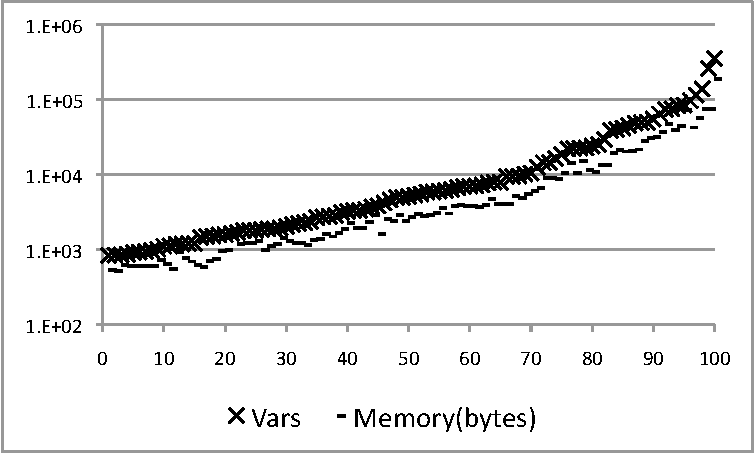
\includegraphics[width=\columnwidth]{images/MemCorr}
\end{center}
\caption{\label{fig:MemCorr}
Comparison between program size (number of var nodes in constraint
graphs) and memory consumption (KB).
Coefficient of determination = 0.9947.
}
\end{figure}

\noindent
\textbf{Precision.}
Our implementation of range analysis is remarkably precise, considering its
runtime.
Lakhdar {\em et al.}'s relational analysis~\cite{Lakhdar11}, for instance, takes
about 25 minutes to go over a program with almost 900 basic blocks.
We analyze programs of similar size in less than one second.
We do not claim our approach is as precise as such algorithms, even though we
are able to find exact bounds to 4/5 of the examples presented
in~\cite{Lakhdar11}.
On the contrary, we present a compromise between precision and speed
that scales to very large programs.
Nevertheless, our results are far from being trivial.
We have implemented a dynamic profiler that measures, for each variable,
its upper and lower limits, given an execution of the target program.
Figure~\ref{fig:precision} compares our results with those measured
dynamically for the Stanford benchmark suite, which is publicly
available~\footnote{\url{http://classes.engineering.wustl.edu/cse465/docs/BCCExamples/stanford.c}}.
We chose Stanford because these benchmarks do not read data from external
files; hence, imprecisions are due to library functions that we cannot
analyze.

\begin{figure}[t!]
\begin{center}
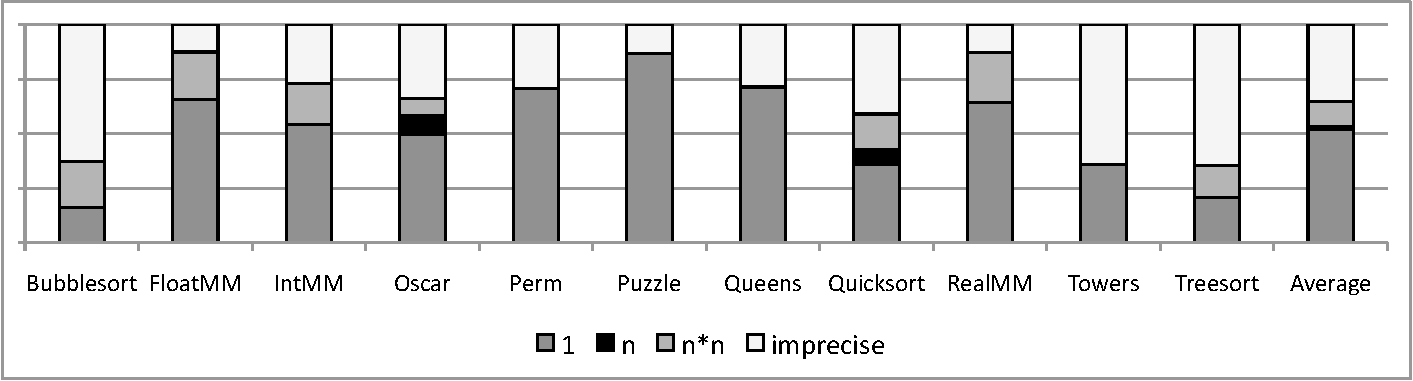
\includegraphics[width=\columnwidth]{images/precUpperBound}
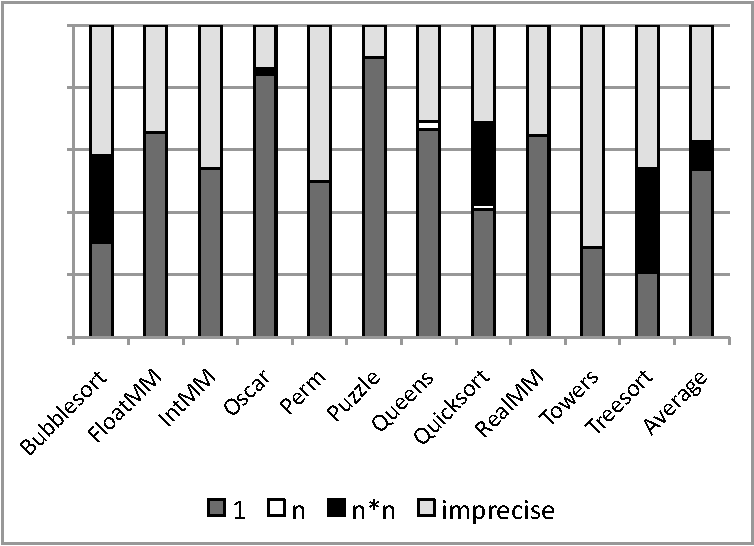
\includegraphics[width=\columnwidth]{images/precLowerBound}
\end{center}
\caption{\label{fig:precision}
(Upper) Comparison between static range analysis and dynamic profiler for
upper bounds.
(Lower) Comparison between static range analysis and dynamic profiler for
lower bounds. The numbers above the benchmark names give the number of
variables in each program.}
\end{figure}

We have classified the bounds estimated by the static analysis into four
categories.
The first category, which we call $1$, contains those bounds that are tight:
during the execution of the program, the variable has been assigned an upper,
or lower limit, that equals the limit inferred statically.
The second category, which we call $n$, contains the bounds that are
within twice the value inferred statically.
For instance, if the range analysis estimates that a variable $v$ is in the
range $[0, 100]$, and during the execution the dynamic profiler finds that
its maximum value is $51$, then $v$ falls into this category.
The third category, $n^2$, contains variables whose actual value is within
a quadratic factor from the estimated value.
In our example, $v$'s upper bound would have to be at most $10$ for it to
be in this category.
Finally, the fourth category contains variables whose estimated value lays
outside a quadratic factor of the actual value.
We call this category {\em imprecise}, and it contains mostly the limits that
our static analysis has marked as either $+\infty$ or $-\infty$.
As we see in Figure~\ref{fig:precision}, 54.11\% of the lower limits that
we have estimated statically are exact.
Similarly, 51.99\% of our upper bounds are also tight.
The figure also shows that, on average, 37.39\% of our lower limits are
imprecise, and 35.40\% of our upper limits are imprecise.
This result is on pair with those obtained by more costly analysis, such as
Stephenson {\em et al.}'s~\cite{Stephenson00}.

\section{Related Work}
\label{sec:rel}

\noindent
\paragraph{Dynamic Detection of Integer Overflows: }
Brumley {\em et al.}~\cite{Brumley07} have developed a tool, RICH, to detect
integer integer overflows.
Their approach consists in instrumenting every integer operation that might cause
to an overflow, underflow, or data loss.
Different from our method, RICH uses specific features of the x86 architecture
to reduce the instrumentation overhead.
Moreover, no static analysis is used to avoid unnecessary assertions, although
this improvement is cited as future work.

\paragraph{Static Detection of Integer Overflows: }
\noindent
Zhang {\em et al.}~\cite{Zhang09} have designed a static analysis to sanitize
programs against integer overflow based vulnerabilities.
They instrument integer operations in paths from a source to a sink.
In Zhang {\em et al.}'s context, sources are functions that read values from
users, and sinks are memory allocation operations.
Thus, contrary to our work, Zhang {\em et al.}'s only need to instrument
about 10\% of the integer operations in the program.
However, they do not use any form of range analysis to limit the number of
checks inserted in the transformed code.
Wang {\em et a.}~\cite{Wang09} have implemented a tool, IntScope, that combines symbolic execution and taint analysis to detect integer overflow vulnerabilities. The authors have been able to use this tool to successfully identify many vulnerabilities in industrial quality software. Our work, and Wang {\em et a.}�s work are essentially different: they use symbolic execution, whereas we rely on
range analysis.
Furthermore, contrary to them, we do not try to detected statically the
possibility of an integer overflow happening.
Contrary to us, they do not transform the program to prevent or detect such event dynamically.
Still in the field of symbolic execution, Molnar
{\em et al.}~\cite{Molnar09} have implemented a tool, SmartFuzz, that analyzes
Linux x86 binaries to find integer overflow bugs.
They prove the existence of bugs by generating test cases for them.

\noindent
\paragraph{Intermediate Program Representations: }

\section{Final Remarks}
\label{sec:rem}

\bibliographystyle{plain}
\bibliography{../references}

\end{document}
